\chapter{Introduction}
\label{sec:introduction}

Wesley -
One more point about the introduction. It should introduce your thesis topic.
It should explain how your topics fit into or expand the standard model and
how your topic(s) enhance our understanding beyond what preceded. You
need to cover both the theoretical and experimental context (e.g. include
a summary of the measurements that came before).

Dasu - 
As a hint, the intro should be accessible to non specialist. So, keep it simple, written in English rather than CMSish. You should introduce SM as the most well tested theory of nature at the fundamental level. The Higgs boson completes it.



The Standard Model (SM) of physics is a mathematical framework for explaining
the interactions and behavior of the fundamental particles observed in nature.
It has been built up and defined through the 1950s and 60s culminating in the
theoretical prediction of the existance of a neutral scalar boson, now called the
Higgs boson.
The SM incorporates descriptions of three of the four fundamental forces of nature:
the strong force, the electromagnetic force, and the weak force.
The force which is not described in the SM is the gravitational force. This omission is one of the reasons
physicists are working to both develop and experimentally test more comprehensive 
theories of nature.

For 40 XXX years after the establishement of the
theoretical prediction of the Higgs boson, the Higgs boson eluded conclusive
observation by experimental particle physicsts. The Higgs boson was discovered in 2012 XXX
by the CMS and ATLAS collaborations at CERN XXX.
With this discovery, all particles predicted and described in the SM have been observed.
Based on research leading up to today, the SM is the most well tested theory of nature at the fundamental level.
Over all, the SM shows remarkable continuity between the theoretical predictions and
the experimental observations. 

Reflecting on the discovery of the Higgs boson, the focus of the experimental particle physics community has transitioned from
Higgs boson ``discovery'' mode to Higgs boson ``measurement'' mode. The leading high energy particle physics experiments
are dedicating a vast portion of their research effort and person power towards
efforts to measure the Higgs boson properties as precisely as possible. Many details of the properties of the Higgs
boson are firmly predicted by theory. Affirmation or negation of these predictions,
such as how often a Higgs boson decays into a pair of $\Pgt$ leptons,
are critical to further testing the merits of the SM. Affirmation of the
predicted Higgs boson properties would further support the SM along with the myriad previous
experimental results. Significant discrepancies between the SM
theoretical predictions and the observed Higgs boson properties could point to
flaws in the SM and would lead to a more full and complete understanding of nature.



\section{The Standard Model of Particle Physics}
The Standard Model of particle physics~\cite{Glashow:1961tr,SM1,SM3} is currently
the best framework for mathematical predictions and explanations of the behavior
of the fundamental particles of nature. These fundamental particles can be grouped
together by behavoir and common characteristis and arranged diagramatically as in
Figure~\ref{fig:sm_particles}. The particles are split vertically into two categories:
fermions which have $\frac{1}{2}$ integer spin, and the bosons which have integer
spin of either 0 or 1. In general, the fermions constitute what we are familiar of
as matter while the bosons are the mediators of the fundamental forces.

\begin{figure*}[htbp]
\centering
     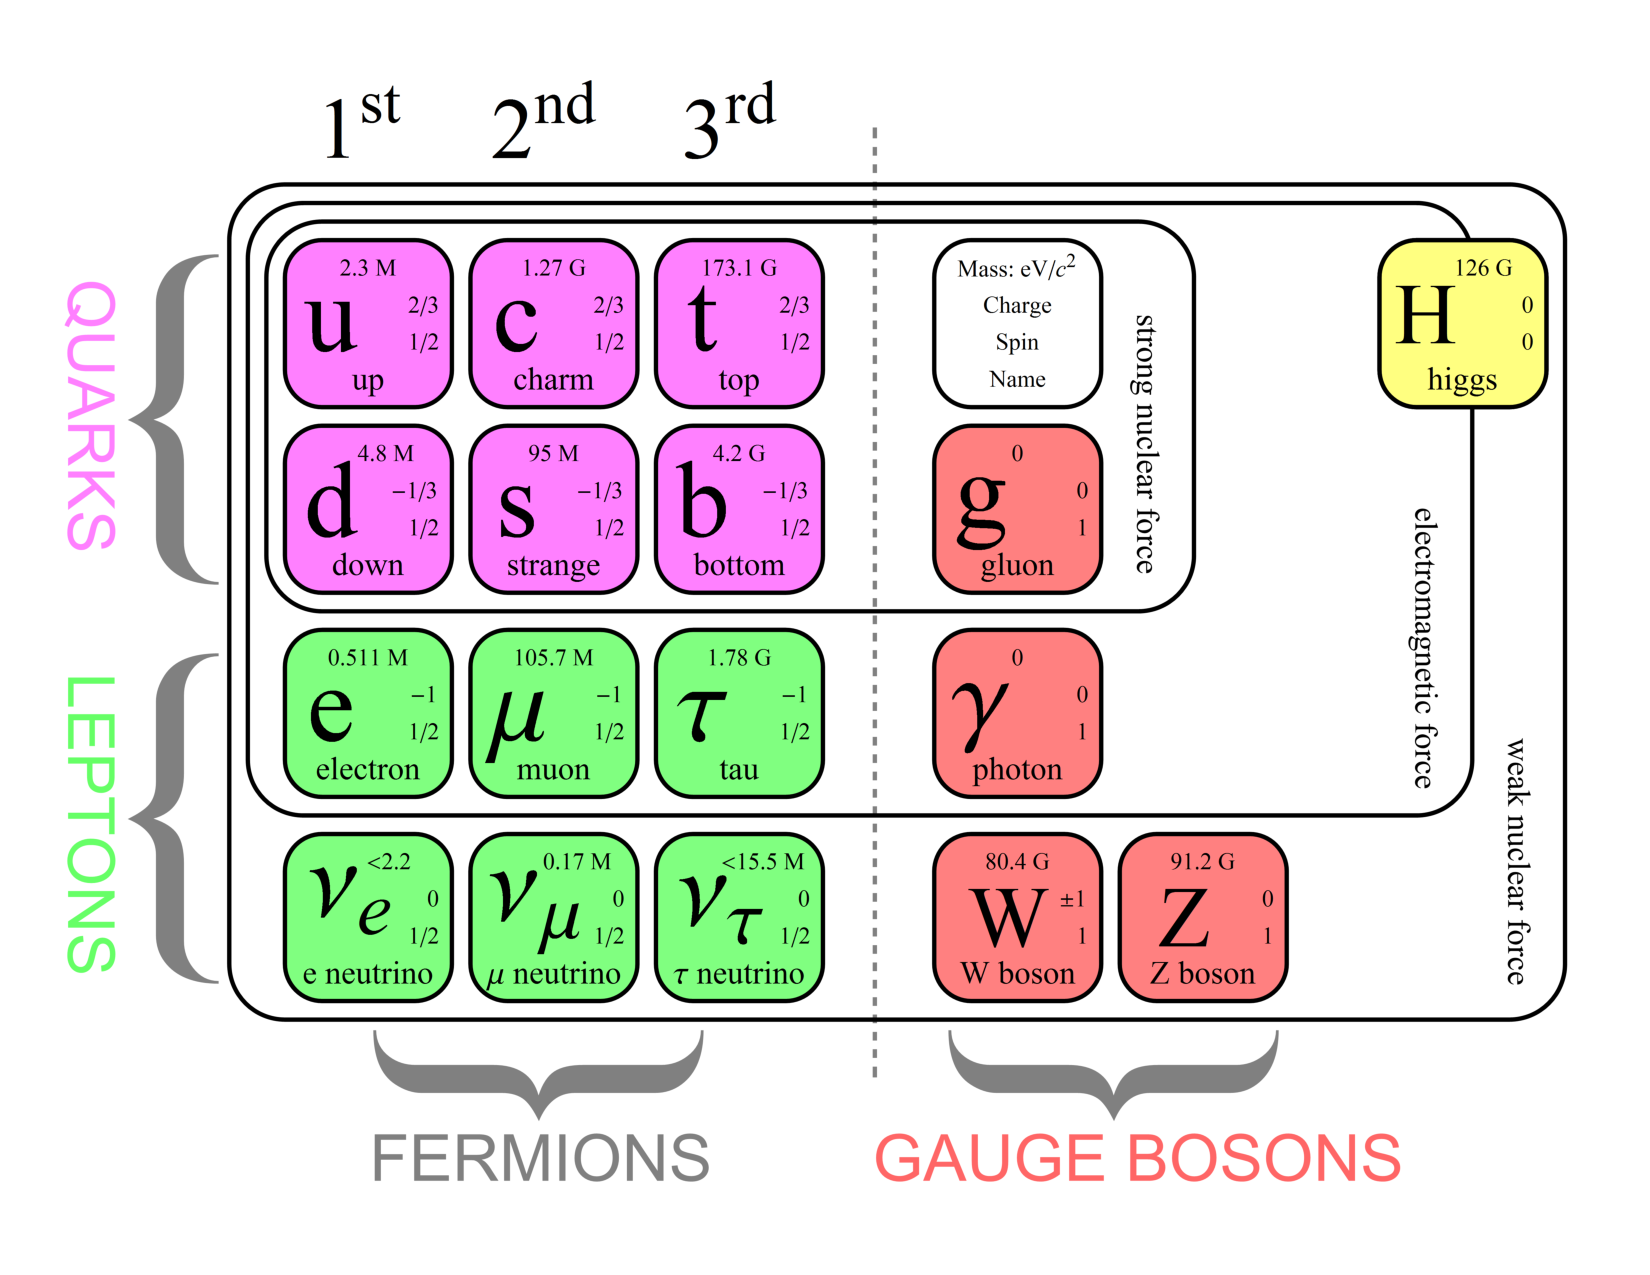
\includegraphics[width=0.7\textwidth]{introduction/plots/sm_particles.pdf}
     \caption{
The fundamental particles of the SM and some of their properties including their:
mass, charge, and spin. The units for mass are reported as electron volts divided by
the speed of light ($c$) squared and use scientific notation prefixes.
M for million, G for billion.
     }
     \label{fig:sm_particles}
\end{figure*}

The fermions can be further grouped into either quarks or leptons based on whether
they carry ``color'' charge or not. 
Quarks carry a color charge and have a charge of either $\frac{-1}{3}$ or $\frac{2}{3}$. 
Where as the leptons are colorless (carry no color charge) and
have integer charge of 0 or -1. In Figure~\ref{fig:sm_particles} the fermions are
arranged according to what is called their mass ``generation'' with more massive
particles appearing to the right in the third mass generation column.

The first
mass generation column composes the fundamental particles which we interact with
every day. Up-quarks and down-quarks are the fundmanetal piecies within
the protons and neutrons building the atoms which contribute to the molecules which
make up the paper pages of this thesis or your computer screen. High energy protons
are a little different and are discussed later in the thesis. Electrons are the
remaining fundamental particles we are familiar with and are also part of the basic 
structure of atoms. The electron neutrino is less familiar because it only
interacts with the other particles through the weak force and does not directly
contribute to the basic atoms which compose the matter from which we are built.

The bosons are split into two groups, the gauge bosons which mediate the three fundamental
forces covered by the SM, and the solo Higgs boson which behaves differently
and will be discussed in detail later. 
The fundamental forces, their mediator particles, and the relative strength of the force
are listed in Table~\ref{tab:sm_forces}. The relatively weak strength of the gravitational
force is what allows the SM to still successfully predice the most basic behaviors
of particles despite not including the gravitational force.

\begin{table*}[htbp]
\centering
\begin{tabular}{lcc}
Fundamental Force        &    Force Mediator             & Relative Strength   \\
\hline
Strong                   &    gluon ($\Pg$)              &   1                 \\ 
Electromagnetic          &    photon ($\Pgg$)            &   $10^{-3}$         \\ 
Weak                     &    $\PW$ and $\PZ$ bosons     &   $10^{-14}$        \\ 
Gravitational            &    unknown                    &   $10^{-43}$        \\ 
\hline
\end{tabular}
\caption{
The fundamental forces, their mediator particles, and the relative strength of the force.
There has been no observed mediator for the gravitational force.
}
\label{tab:sm_forces}
\end{table*}

The strong force has the largest relative strength of the fundamental forces but
the reach or distance over which the force can be felt is very limited and is 
confined to the sub-atomic scale, $10^{-15} m$. The strong force is experienced
between particles with a color charge, exclusively gluons and quarks.

The electromagnetic force follows after the strong force for largest relative
strength. The reach of the electromagnetic force is infinite and decreases with
distance as $\frac{1}{r^{2}}$. Despite its infinite reach, the electromagnetic 
force is not experienced on the macro scale because all stable matter is composed
of equal parts positively charged matter and negatively charged matter leading to
a neutrally charged universe. The electromagnetic force is experienced by all
charged particles XXX XXX XXX

\begin{figure*}[htbp]
\centering
     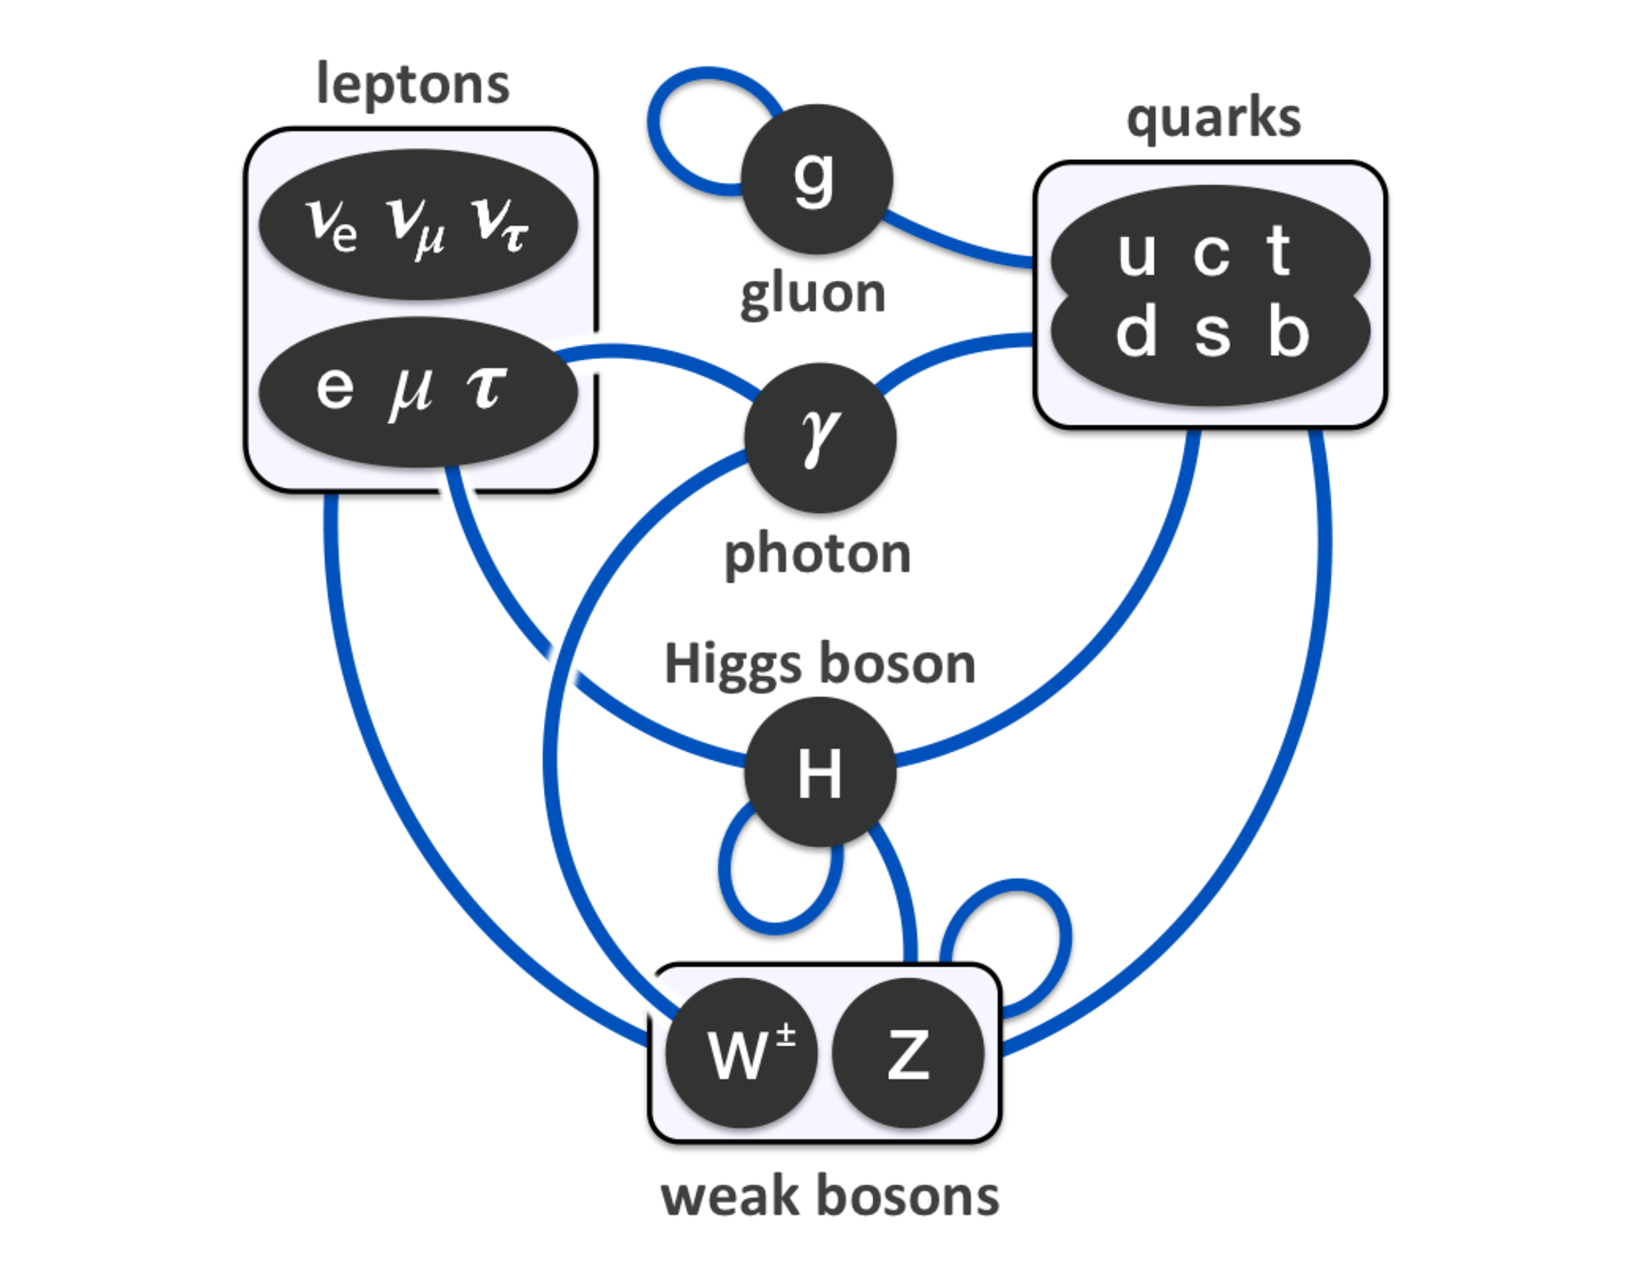
\includegraphics[width=0.7\textwidth]{introduction/plots/elementary_particle_interactions_SM.pdf}
     \caption{
Diagram showing the bosons arranged into a central column with the fermions in the
upper corners. The blue lines linking particles and groups of particles together
indicate that those fermions can be influenced by force associated to that mediator
boson. The Higgs boson in the center is discussed in Chapter~\ref{sec:pheno}.
     }
     \label{fig:sm_particles}
\end{figure*}



Anti-particles


electroweak symmetry breaking is achieved via the Brout--Englert--Higgs
mechanism~\cite{Englert:1964et,Higgs:1964ia,Higgs:1964pj,Guralnik:1964eu,Higgs:1966ev,Kibble:1967sv},
leading, in its minimal version, to the prediction of the existence of one physical neutral scalar particle,
commonly known as the Higgs boson ($\PH$).









To establish the mass generation mechanism for fermions,
 it is necessary to probe the direct coupling of
the Higgs boson to such particles.
The most promising decay channel is $\Pgt^+\Pgt^-$,
because of the large event rate expected in the SM compared to the $\Pgm^+\Pgm^-$ decay channel ($\mathcal{B}(\PH\to\Pgt^+\Pgt^-)=6.3$\% for a mass of 125.09\GeV), and of the smaller contribution from background events
with respect to the $\bbbar$ decay channel.

\subsection{Electroweak Symmetry Breaking}

\subsubsection{W/Z Higgs Associated Production}

\subsection{Cross Sections and Decay Rates}

\subsection{QCD and Proton Structure}

\section{Experimental Context: Previous Higgs Measurements}

\subsection{CMS and ATLAS at 7 and 8 TeV}
A particle compatible with such a boson was observed by the ATLAS and CMS experiments at the CERN LHC
in the $\PZ\PZ$, $\Pgg \Pgg$, and $\PW\PW$ decay channels~\cite{Aad:2012tfa, Chatrchyan:2012xdj, Chatrchyan:2013lba},
during the proton-proton ($\Pp\Pp$) data taking period in 2011 and 2012
at center-of-mass energies of $\sqrt{s} = 7$ and 8\TeV, respectively.
Subsequent results from both experiments, described in
Refs.~\cite{Aad:2015gba, Khachatryan:2014jba, Chatrchyan:2012jja, Aad:2013xqa, Khachatryan:2014kca,Sirunyan:2017exp},
established that the measured properties of the new particle,
including its spin, CP properties,
and coupling strengths to SM particles, are consistent with those expected for the Higgs boson predicted by the SM.
The mass of the Higgs boson has been determined to be
$125.09\pm0.21\stat\pm0.11\syst\GeV$, from a combination of
ATLAS and CMS measurements~\cite{Aad:2015zhl}.

Searches for a Higgs boson decaying to a $\Pgt$ lepton pair were performed at the LEP~\cite{Barate:2000ts,Abdallah:2003ip,Achard:2001pj,Abbiendi:2000ac},
Tevatron~\cite{Aaltonen:2012jh, Abazov:2012zj}, and LHC colliders.
Using $\Pp\Pp$ collision data at $\sqrt{s}=7$ and $8\TeV$, the CMS Collaboration showed evidence for this process with an observed\,(expected)
significance of 3.2\,(3.7) standard deviations (s.d.)~\cite{Chatrchyan:2014nva}. The ATLAS
experiment reported evidence for Higgs bosons decaying into pairs
of $\Pgt$ leptons with an observed (expected) significance of 4.5 (3.4)
s.d. for a Higgs boson mass of 125\GeV~\cite{Aad:2015vsa}.
The combination of the results from both experiments yields an observed (expected)
significance of 5.5\,(5.0) s.d.~\cite{Khachatryan:2016vau}.








